\documentclass[a4paper]{article}

%% Language and font encodings
\usepackage[english]{babel}
\usepackage[utf8x]{inputenc}
\usepackage[T1]{fontenc}
\usepackage{cite}

\usepackage{graphicx}
\usepackage{subcaption}
\usepackage{tikz}
\usepackage{pgfplots}
\usepackage{wrapfig}
\usepackage{cutwin}
\graphicspath{ {images/} }
\usetikzlibrary{intersections,decorations.pathreplacing,decorations.markings,calc}

%% Sets page size and margins
\usepackage[a4paper,top=3cm,bottom=2cm,left=2cm,right=2cm,marginparwidth=1.75cm]{geometry}

%% Useful packages
\usepackage{amsmath}
\usepackage{amsthm}
\usepackage{amssymb}
\usepackage{tikz}
\usepackage{graphicx}
\usepackage{hyperref}
\usepackage{caption}
%\usepackage{subcaption}
\usepackage{float}
\captionsetup{font={small,it}}
\theoremstyle{definition}
\newcommand{\D}{\mathbb{D}}
\newcommand{\Z}{\mathbb{Z}}
\newcommand{\R}{\mathbb{R}}
\newcommand{\C}{\mathcal{C}}
\newcommand{\A}{\mathcal{A}}
\newcommand{\B}{\mathcal{B}}
\newcommand{\dx}{\: \mathrm{d}}
\newcommand{\Scrystal}{\mathcal{S}_D^\#}
\newcommand{\KstarC}{(\mathcal{K}_D^{\#})^*}
\newcommand{\expl}[1]{\left[\text{\footnotesize \emph{#1}} \right]}
\newcommand{\ds}{\displaystyle}
\newcommand{\eqnref}[1]{(\ref {#1})}
\def\nm{\noalign{\medskip}}



\author{Erik Orvehed Hiltunen}

\begin{document}
\section{Introduction}
We consider acoustic wave propagation in a crystal with bubbles repeated in a periodic square lattice. It has previously been shown that such crystal exhibits a frequency bandgap, so waves with frequencies inside this bandgap will decay exponentially. By perturbing one bubble to have a resonance frequency inside the bandgap, we expect a localized mode inside the crystal. 


\section{Problem statement}
Assume that a single bubble occupies $D$, which is a circle of radius $R_b$ and center at the origin. Let $\C = \cup_{n\in\Z^2}(D+n)$ be the periodic bubble crystal.

Consider now a perturbed crystal, where $D$ is replaced by a defect circle $D_d$ of radius $R_d < R_b$. Let $\C_d = D_d \cup \left( \cup_{n\in\Z^2\setminus\{0,0\}} D+n \right)$ be the perturbed crystal. We consider the following problem
\begin{equation} \label{eq:scattering}
\left\{
\begin{array} {ll}
	&\ds \nabla \cdot \frac{1}{\rho} \nabla  u+ \frac{\omega^2}{\kappa} u  = 0 \quad \text{in} \quad \R^2 \backslash \C_d, \\
	\nm
	&\ds \nabla \cdot \frac{1}{\rho_b} \nabla  u+ \frac{\omega^2}{\kappa_b} u  = 0 \quad \text{in} \quad \C_d, \\
	\nm
	&\ds  u_{+} -u_{-}  =0   \quad \text{on} \quad \partial \C_d, \\
	\nm
	& \ds  \frac{1}{\rho} \frac{\partial u}{\partial \nu} \bigg|_{+} - \frac{1}{\rho_b} \frac{\partial u}{\partial \nu} \bigg|_{-} =0 \quad \text{on} \quad \partial \C_d
\end{array}
\right.
\end{equation}
Here, $\partial/\partial \nu$ denotes the outward normal derivative and $|_\pm$ denote the limits from outside and inside $D$.  

Let
\begin{equation*} % \label{data1}
v = \sqrt{\frac{\kappa}{\rho}}, \quad v_b = \sqrt{\frac{\kappa_b}{\rho_b}}, \quad k= \frac{\omega}{v} \quad \text{and} \quad k_b= \frac{\omega}{v_b}
\end{equation*}
be respectively the speed of sound outside and inside the bubbles, and the wavenumber outside and inside the bubbles. We also introduce two dimensionless contrast parameters
\begin{equation*} % \label{data2}
\delta = \frac{\rho_b}{\rho} \quad \text{and} \quad \tau= \frac{k_b}{k}= \frac{v}{v_b} =\sqrt{\frac{\rho_b \kappa}{\rho \kappa_b}}. 
\end{equation*}

Let $G(x,y)$ be the Green's function corresponding to the periodic crystal, i.e. $G$ satisfies
\begin{equation*} \label{eq:G}
\Delta G + (k^2+(k_b^2-k^2)\chi(\C))G = \delta(x-y)
\end{equation*}
Let $\Gamma^k$ be the fundamental solution to the Helmholtz equation with wavenumber $k$ and $\mathcal{S}_{D}^k$ be the free-space single layer potential defined by
\begin{equation*}
\mathcal{S}_D^k[\phi](x) = \int_{\partial D} \Gamma^k(x,y)\phi(y) \dx \sigma(y), \quad x \in \R^2,
\end{equation*}
Let $\Scrystal$ be the single layer potential associated to the Green's function $G$, i.e.
\begin{equation*}
\Scrystal[\phi](x) = \int_{\partial D} G(x,y)\phi(y) \dx \sigma(y) , \quad x \in \R^2.
\end{equation*}

We seek a solution $u(x)$ of the form
\begin{equation} \label{eq:sol}
u(x) = \begin{cases}
\mathcal{S}_{D_d}^{k_b}[\phi_1](x) \quad &x\in D_d \\
\mathcal{S}_{D_d}^{k}[\phi_2](x) + S_D^k[\phi_3](x) & x\in D\setminus D_d \\
\Scrystal[\phi_4](x) & x \in \R^2\setminus D.
\end{cases}
\end{equation}
A solution of this form satisfies the differential equation in \eqnref{eq:scattering}. To write the boundary conditions in equation \eqnref{eq:scattering} in therms of the boundary integral operators, we need the jump relations for the single layer potentials. For $S_D^k$, these are well known, but it remains to compute these for $S_D^\#$.

\subsection{Jump relations for $S_D^\#$}
For $x$ close to $y$ on the boundary of a bubble, $|x-y|$ is small compared to the wavelength so we are in the quasi-static regime. We therefore expect the singularity of $G$ to be the same as the singularity of the Laplace Green's function $G_0(x,y)$, which is the solution to 
\begin{equation*}
\left\{
\begin{array}{ll}
	&\ds \Delta G_0 = \delta(x-y) \quad \text{in}\quad \R^2 \\
	&\ds \frac{1}{\rho}\frac{\partial G_0}{\partial \nu}\bigg|_+ - \frac{1}{\rho}\frac{\partial G_0}{\partial \nu}\bigg|_- = 0 \quad \text{in} \quad \partial D \\
	&\ds G_0 \text{ satisfies Sommerfeld radiation condition} 
\end{array}
\right.	
\end{equation*}
Set $\tilde{G}_0 = G_0-\Gamma^0$, where $\Gamma^0(x,y)= \frac{-1}{2\pi}\ln(|x-y|)$ is the fundamental solution for the Laplace equation in $\R^2$. Then $\tilde{G}_0$ is the solution to the following conductivity problem
\begin{equation*}
\left\{
\begin{array}{ll}
&\ds \Delta \tilde{G}_0 = 0 \quad \text{in}\quad \R^2 \\
&\ds G_0\big|_+-G_0\big|_- = 0 \\
&\ds \frac{1}{\rho}\frac{\partial \tilde{G}_0}{\partial \nu}\bigg|_+ - \frac{1}{\rho}\frac{\partial \tilde{G}_0}{\partial \nu}\bigg|_- = (1-\delta)\frac{\partial \Gamma^0}{\partial \nu} \quad \text{in} \quad \partial D \\
&\ds \tilde{G}_0 \text{ satisfies Sommerfeld radiation condition} 
\end{array}
\right.	
\end{equation*}
It is well known that the solution to this problem is given by
\begin{equation*}
\tilde{G}(x,y) = \mathcal{S}_D^0 \left[\psi\right](x),
\end{equation*}
where
\begin{equation*}
\psi(z) = \left(\lambda I - \left( \mathcal{K}_D^0 \right)^*\right)^{-1} \left[ \frac{\partial\Gamma^0(z,y)}{\partial \nu(z)} \right] 
\end{equation*}
For a disk $D$, the operator $\left(\mathcal{K}_D^0\right)^*$ has an explicit expression
\begin{equation*}
\left(\mathcal{K}_D^0\right)^*[\phi](x) = \frac{1}{4\pi R_b}\int_{\partial D} \phi(y)\dx \sigma,
\end{equation*}
valid for all $x\in \partial D$. Furthermore, $\mathcal{K}_D^0$ is self-adjoint in this case. For $y$ outside $D$ the function $\Gamma^0(x,y)$ is harmonic as a function of $x\in D$. Therefore 
\begin{equation*}
\int_{\partial D} \frac{\partial \Gamma^0(x,y)}{\partial(x) \nu}\dx \sigma(x) = 0,
\end{equation*}
so it can easily be shown that 
\begin{equation*}
\int_{\partial D} \psi(x)\dx \sigma = 0,
\end{equation*}
and hence 
\begin{equation*}
\psi = \frac{1}{\lambda}\frac{\partial \Gamma^0}{\partial \nu}.
\end{equation*}
It follows that 
\begin{align*}
\tilde{G}(x,y) &= \frac{1}{\lambda}\mathcal{S}_D^0 \left[\frac{\partial \Gamma^0(z,y)}{\partial \nu(z)} \right](x) \\
&= \frac{1}{\lambda} \int_{\partial D} \Gamma^0(x,z) \frac{\partial \Gamma^0(z,y)}{\partial \nu(z)} \dx \sigma(z) \\
&=\frac{1}{\lambda}\mathcal{D}_D^0 \left[\Gamma^0(z,x)\right](y)
\end{align*}
Taking the limit $y\rightarrow \partial D+$ and using the jump relation for the double layer potential $\mathcal{D}_D^0$, we find
\begin{equation*}
\tilde{G}_0(x,y) = -\frac{\Gamma^0(x,y)}{2\lambda} + \frac{1}{\lambda}\mathcal{K}_D^0\left[\Gamma^0(x,z)\right](y).
\end{equation*}
Here $\mathcal{K}_D^0\left[\Gamma^0(x,z)\right](y)$ is a bounded constant $C(x)$ with respect to $y$ (and actually equals $\frac{1}{2}\Gamma^0(x,0)$). Plugging into the formula for $G$ we find
\begin{equation*}
G(x,y) = c\Gamma^0(x,y) + C(x),
\end{equation*}
where 
\begin{equation*}
c = \frac{2}{\delta+1}.
\end{equation*}

\subsection{Boundary integral formulation}
Implies that the layer densities $\phi_i,\ i=1,2,3,4$ satisfies the system of boundary integral equations $\A(\omega, \delta)\Phi = 0$, where
\begin{equation} \label{eq:A}
\A(\omega, \delta) = 
\begin{pmatrix}
\mathcal{S}_{D_d}^{k_b} &  -\mathcal{S}_{D_d}^{k} & -\mathcal{S}_{D_d,D}^{k} & 0 \\
0 & \mathcal{S}_{D,D_d}^k & \mathcal{S}_{D}^k & -\Scrystal \\
-\frac{1}{2}I+ (\mathcal{K}_{D_d}^{k_b})^*& -\delta\left( \frac{1}{2}I+ (\mathcal{K}_{D_d}^{k})^*\right) & -\delta \frac{\partial \mathcal{S}_{D_d,D}^{k}}{\partial \nu} & 0 \\
0 & \frac{\partial \mathcal{S}_{D,D_d}^{k}}{\partial \nu} & -\frac{1}{2}I+ (\mathcal{K}_D^{k})^* & -\left( \frac{1}{2}I+ \KstarC\right)
\end{pmatrix}, 
\ \text{and}  \ \Phi= 
\begin{pmatrix}
\phi_1\\
\phi_2 \\
\phi_3 \\
\phi_4
\end{pmatrix}.
\end{equation}
Here the operator $\mathcal{S}_{D_d,D}^{k} = \mathcal{S}_{D}^{k}|_{x\in \partial D_d}$ is the restriction of $\mathcal{S}_{D}^{k}$ onto $\partial D_d$.

\section{Simplified problem}
By perturbing the size of one bubble, we expect one localized mode, which quickly decays away from the perturbed bubble. To model this behavior, we first consider a simpler problem. Intuitively, the exponential decay means that the solution $u(x)$ is close to zero for $x$ large enough. In this simplified problem, we assume that $u(x)=0$ for $|x|=R_b$, i.e. for $x$ on the large bubble $D$, and only consider the problem inside $D$. We therefore consider the Dirichlet problem
\begin{equation} \label{eq:simple}
\left\{
\begin{array} {ll}
&\ds \nabla \cdot \frac{1}{\rho} \nabla  u+ \frac{\omega^2}{\kappa} u  = 0 \quad \text{in} \quad D \backslash D_d, \\
\nm
&\ds \nabla \cdot \frac{1}{\rho_b} \nabla  u+ \frac{\omega^2}{\kappa_b} u  = 0 \quad \text{in} \quad D_d, \\
\nm
&\ds  u_{+} -u_{-}  =0   \quad \text{on} \quad \partial D_d, \\
\nm
& \ds  \frac{1}{\rho} \frac{\partial u}{\partial \nu} \bigg|_{+} - \frac{1}{\rho_b} \frac{\partial u}{\partial \nu} \bigg|_{-} =0 \quad \text{on} \quad \partial D_d \\
&\ds u_- = 0 \quad \text{on} \quad \partial D.
\end{array}
\right .
\end{equation}
We seek the resonance frequencies, i.e. the frequencies $\omega$ such that equation \eqnref{eq:simple} has a non-trivial solution. This problem is solved numerically using two different methods. Similarly to equation \eqnref{eq:sol}, we seek a solution of the form 
\begin{equation} \label{eq:simplesol}
u(x) = \begin{cases}
\mathcal{S}_{D_d}^{k_b}[\phi_1](x) \quad &x\in D_d \\
\mathcal{S}_{D_d}^{k}[\phi_2](x) + S_D^k[\phi_3](x) & x\in D\setminus D_d,
\end{cases}
\end{equation}
satisfying $\tilde{\A}(\omega, \delta)\Phi = 0$, where
\begin{equation} \label{eq:simpleA}
\tilde{\A}(\omega, \delta) = 
\begin{pmatrix}
\mathcal{S}_{D_d}^{k_b} &  -\mathcal{S}_{D_d}^{k} & -\mathcal{S}_{D_d,D}^{k} \\
0 & \mathcal{S}_{D,D_d}^k & \mathcal{S}_{D}^k \\
-\frac{1}{2}I+ (\mathcal{K}_{D_d}^{k_b})^*& -\delta\left( \frac{1}{2}I+ \left(\mathcal{K}_{D_d}^{k}\right)^*\right) & -\delta \frac{\partial \mathcal{S}_{D_d,D}^{k}}{\partial \nu}
\end{pmatrix}, 
\ \text{and}  \ \Phi= 
\begin{pmatrix}
\phi_1\\
\phi_2 \\
\phi_3
\end{pmatrix}.
\end{equation}
The integral operators in $\tilde{\mathcal{A}}$ are discretized using Nyström's method and the smallest resonance frequency is computed using Muller's method. \cite{first}

To verify the solution, the problem is also solved using multipole expansions. Because the problem is a radially symmetric Helmholtz problem, the solution $u(x)$ can be written
\begin{equation*}
u(x) = \begin{cases}
\sum_{n=-\infty}^\infty a_n J_n(k_br)e^{in\theta} \quad &\text{if } r<R_d \\
\sum_{n=-\infty}^\infty \left(b_n J_n(kr) + c_n H^{(1)}_n(kr)\right) e^{in\theta}  &\text{if } r>R_d.
\end{cases}
\end{equation*}
Using the boundary conditions, we find that for every $n\in \Z$,
\begin{equation*} 
\begin{pmatrix}
J_n(k_bR_d) &  -J_n(kR_d) & -H_n^{(1)}(kR_d) \\
k_bJ_n'(k_bR_d) & -\delta kJ_n'(kR_d) & -\delta k H^{(1)'}_n(kR_d)\\
0 & J_n(kR_b) & H^{(1)}_n(kR_b)
\end{pmatrix}
\begin{pmatrix}
a_n \\ b_n \\ c_n
\end{pmatrix} = 0.
\end{equation*}
We therefore seek the $\omega$ such that for some $n$, this system is not invertible. It is intuitively clear that the first resonant frequency will contain a factor with $n=0$. Thus, the lowest resonant frequency corresponds to the matrix
\begin{equation*} 
\begin{pmatrix}
J_0(k_bR_d) &  -J_0(kR_d) & -H_0^{(1)}(kR_d) \\
k_bJ_0'(k_bR_d) & -\delta kJ_0'(kR_d) & -\delta k H^{(1)'}_0(kR_d)\\
0 & J_0(kR_b) & H^{(1)}_0(kR_b)
\end{pmatrix}
\end{equation*}
being singular. This frequency is computed using Muller's method.
\begin{figure}[H]
	\centering
	\begin{minipage}[t]{0.45\linewidth}
	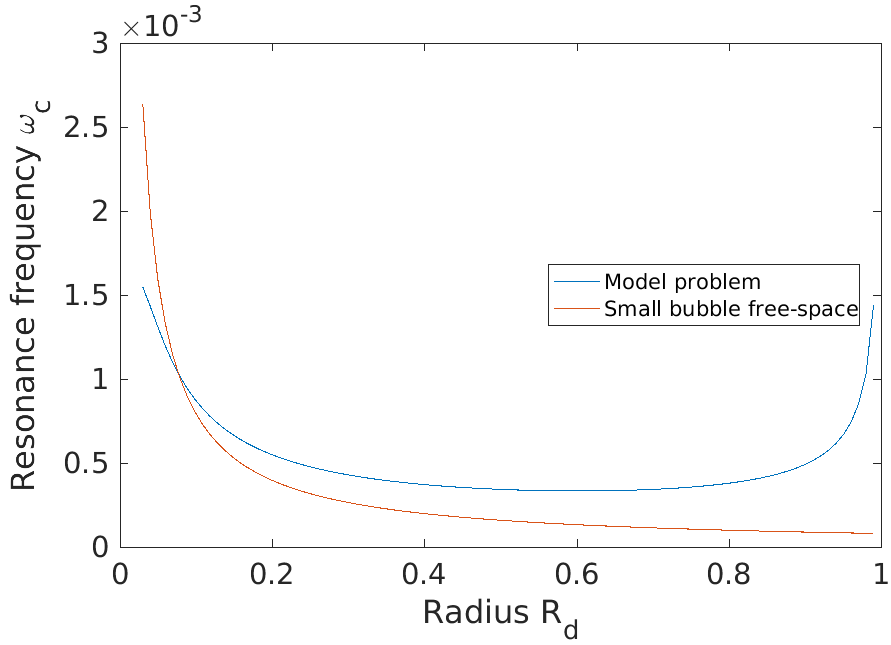
\includegraphics[scale=0.5]{../Model_problem/simpleSol.png}
	\caption{Resonance frequency for different defect radius $R_d$.}
	\label{fig:simpleSol}
	\end{minipage}
	\hspace{10pt}
	\begin{minipage}[t]{0.45\linewidth}
	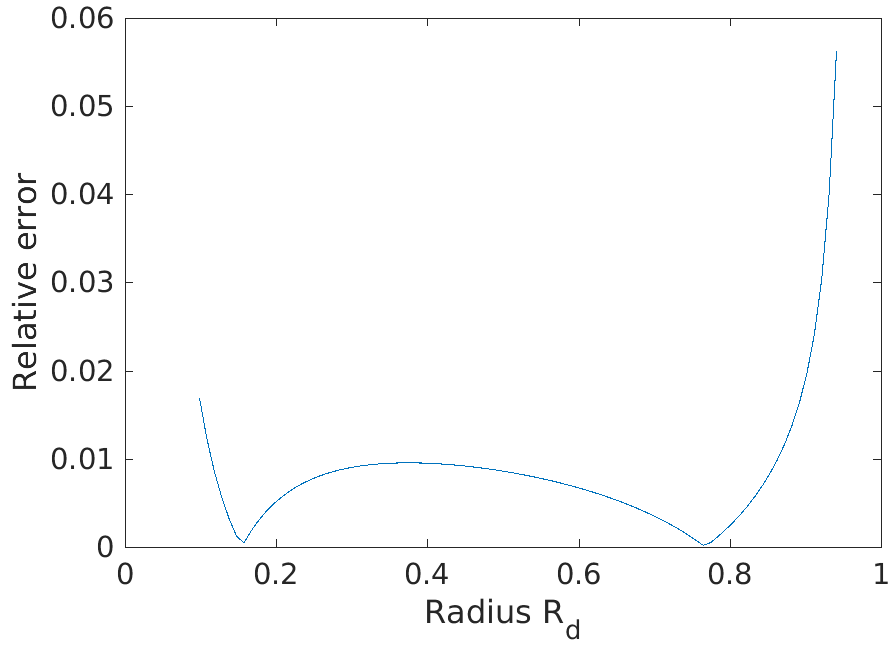
\includegraphics[scale=0.5]{../Model_problem/simpleErr.png}
	\caption{Relative error between integral formulation and multipole expansion solutions for different defect radius $R_d$.}
	\label{fig:simpleErr}
\end{minipage}
\end{figure}

Figure \ref{fig:simpleSol} shows the resonance frequency of the model problem, the resonance frequency of the small bubble in free-space and the resonance frequency of the Dirichlet problem on the big bubble without the inclusion. It can be seen that the resonance frequency of the model problem is higher compared to the bubble in free-space. For $R_d \rightarrow R_b$, the system behaves like a Dirichlet problem for the Helmholtz equation on the small bubble, and the resonance frequency tends to the first eigenvalue of this problem.

Figure \ref{fig:simpleErr} shows the relative error between the solutions using the integral operator and the multipole expansions methods. For intermediate $R_d$, the relative error is of the order $1\%$, so the two methods agree.

The conclusion is that we also have resonance in the model problem, and that the resonance frequency is higher compared to the free-space bubble. This suggests that there will be a resonance mode corresponding to the small bubble in the full problem, and that this resonance frequency will lie in the bandgap of the crystal.

\section{Numerical implementation}
We seek a spatial discretization of the boundary integral formulation. The factors $\Scrystal$ and $\KstarC$ require the Green's function $G$ for the crystal, so the equation \eqnref{eq:G} has to be solved numerically. We will apply the method found in \cite{bandgap}.
Applying the Floquet transform we can decompose $G$ into the $\alpha$-quasiperiodic Green's function $G_\alpha$ which satisfies
\begin{equation*}
\Delta G_\alpha + (k^2+(k_b^2-k^2)\chi(\C))G_\alpha = \sum_{n\in \Z} \delta(x-y-n)e^{in\cdot\alpha}
\end{equation*}
Here $\alpha$ is in the so called first Brillouin zone $[0,2\pi]^2$. Let $Y= [-1/2,1/2]^2$. For a fixed $y\in \R^2$, the function $u(x)=G_\alpha(x,y)$ is a solution to the problem
\begin{equation} \label{eq:quasiperiodic}
\left\{
\begin{array} {ll}
&\ds \nabla \cdot \frac{1}{\rho} \nabla  u+ \frac{\omega^2}{\kappa} u  = \delta(x-y) \quad \text{in} \quad Y \backslash D, \\
\nm
&\ds \nabla \cdot \frac{1}{\rho_b} \nabla  u+ \frac{\omega^2}{\kappa_b} u  = \delta(x-y) \quad \text{in} \quad D, \\
\nm
&\ds  u_{+} -u_{-}  =0   \quad \text{on} \quad \partial D, \\
\nm
& \ds  \frac{1}{\rho} \frac{\partial u}{\partial \nu} \bigg|_{+} - \frac{1}{\rho_b} \frac{\partial u}{\partial \nu} \bigg|_{-} =0 \quad \text{on} \quad \partial D \\
&  e^{-i \alpha \cdot x} u  \,\,\,  \text{is periodic.}
\end{array}
\right.
\end{equation}
Because of the reciprocity relation $G_\alpha(x,y) = G_\alpha(y,x)$, also $e^{-i \alpha \cdot y} G_\alpha(x,y)$ is periodic in $y$, so we can restrict to the case $y\in Y$. Recall that the quasi-periodic Green's function $\Gamma_\alpha^k$, defined as the solution to the equation
\begin{equation*}
\Delta \Gamma_\alpha^k(x,y) + k^2\Gamma_\alpha\alpha^k(x,y) = \sum_{n\in \Z} \delta(x-y-n)e^{in\cdot\alpha}
\end{equation*}
can be expanded as 
\begin{equation} \label{eq:quasihomogenious}
\Gamma_\alpha^k(x,y) = -\frac{i}{4}\sum_{m\in \Z^2} H_0^{(1)}(k|x-y-m|)e^{im\cdot\alpha}
\end{equation}
Then $G_\alpha$ can be written

\begin{equation} \label{eq:G_a}
G_\alpha(x,y) = \begin{cases} \Gamma_\alpha^{k_b}(x,y) + S_D^{k_b}[\psi_b](x) \quad &x\in D \\  \Gamma_\alpha^{k}(x,y) + S_D^{k}[\psi](x) &x\in Y \backslash \bar{D} \end{cases}
\end{equation}
Using the jump relations for the single layer potentials, we find that
\begin{equation*}
\B(\omega,\delta)[\Psi] = F
\end{equation*}
where 
\begin{equation*}
\B(\omega, \delta) = 
\begin{pmatrix}
\mathcal{S}_D^{k_b} &  -\mathcal{S}_D^{\alpha,k}  \\
-\frac{1}{2}+ \mathcal{K}_D^{k_b, *}& -\delta( \frac{1}{2}+ (\mathcal{K}_D^{ -\alpha,k})^*)
\end{pmatrix}, 
\,\, \Psi= 
\begin{pmatrix}
\psi_b\\
\psi
\end{pmatrix},
\,\, F=
\begin{pmatrix}
\Gamma_\alpha^{k} - \Gamma_\alpha^{k_b} \\
\delta\frac{\partial \Gamma_\alpha^{k}}{\partial \nu} -
\frac{\partial \Gamma_\alpha^{k_b}}{\partial \nu} 
\end{pmatrix}
\end{equation*}
The method in \cite{bandgap} uses the Fourier basis $e^{in\theta}$, so  we need to expand the function $\Gamma_\alpha^k(x,y)$ in terms of the polar coordinates $(r,\theta)$ of $x$. We will use the following version of Graf's addition theorem.

\begin{equation*}
H_l^{(1)}(kr_2)e^{il\theta_2} =
\begin{cases}
\sum_{n=-\infty}^\infty H_{l-n}^{(1)}(kb)e^{i(l-n)\beta}J_n(kr_1)e^{in\theta_1} \qquad &\text{if } r_1<b \\
\sum_{n=-\infty}^\infty H_{l-n}^{(1)}(kr_1)e^{i(l-n)\theta_1}J_n(kb)e^{in\beta} \qquad &\text{if } r_1>b
\end{cases}
\end{equation*}
In these equations we have $x_1 = r_1e^{i\theta_1}, x_2 = r_2e^{i\theta_2}$ and $x_2 = x_1 + be^{i\beta}$. 

In the following, pick $x$ on the boundary $\partial D$, i.e. $x = R_be^{i\theta}$. Furthermore, pick $y=r'e^{i\theta'}$ inside $Y$. Using the addition formulas, we have
\begin{align*}
H_0^{(1)}(k|x-y-m|) &= 
\begin{cases}
\sum_{n=-\infty}^\infty (-1)^nH_{-n}^{(1)}(k|y+m|)e^{-in\theta_m'}J_n(kR_b)e^{in\theta} \qquad &\text{if } R_b<|y+m| \\
\sum_{n=-\infty}^\infty (-1)^nH_{-n}^{(1)}(kR_b)e^{-in\theta}J_n(k|y+m|)e^{in\theta_m'} \qquad &\text{if } R_b>|y+m|
\end{cases}
\end{align*}
For $m\neq 0$ we have $R_b<|y+m|$ and
\begin{equation*}
H_{-n}^{(1)}(k|y+m|)e^{-in\theta_m'} = \sum_{l=-\infty}^\infty H_{-n-l}^{(1)}(k|m|)e^{i(-n-l)\theta_m}J_l(kr')e^{il\theta'}
\end{equation*}
Plugging in above expressions into equation \ref{eq:quasihomogenious}, we find
\begin{equation*}
\Gamma_\alpha^k(x,y) = -\frac{i}{4}\sum_{n=-\infty}^\infty\left[ M_ne^{in\theta} + \sum_{l=-\infty}^\infty\left[ \sum_{m\in \Z^2, m\neq 0} H_{-n-l}(k|m|)e^{i(-n-l)\theta_m}e^{im\cdot\alpha} \right] (-1)^nJ_l(kr')e^{il\theta'}J_n(kR_b)e^{in\theta}\right],
\end{equation*}
where the terms $M_n$, corresponding to $m=0$, are given by
\begin{equation*}
M_n = \begin{cases}
(-1)^nH_{-n}(kr')e^{-in\theta'}J_n(kR_b) \quad &\text{if } r' > R_b \\
(-1)^nH_{n}(kR_b)J_{-n}(kr')e^{-in\theta'} \quad &\text{if } r' < R_b.
\end{cases}
\end{equation*}
The two different cases correspond to the source $y$ being inside or outside the bubble. Define the lattice sum $Q_n$ as 
\begin{equation*}
Q_n = \sum_{m\in \Z^2, m\neq 0} H_{n}(k|m|)e^{in\theta_m}e^{im\cdot\alpha}.
\end{equation*}
Then the equation for $\Gamma_\alpha^k$ is 
\begin{equation}\label{eq:gammafourier}
\Gamma_\alpha^k(x,y) = -\frac{i}{4}\sum_{n=-\infty}^\infty\left[ M_n + \sum_{l=-\infty}^\infty Q_{-n-l} (-1)^nJ_l(kr')e^{il\theta'}J_n(kR_b)\right]e^{in\theta}.
\end{equation}
This can be viewed as a Fourier series expansion of $\Gamma_\alpha^k$ as a function of $x\in S^1$. The $n$:th Fourier coefficient is
\begin{equation*}
-\frac{i}{4}\left[M_n + \sum_{l=-\infty}^\infty Q_{-n-l} (-1)^nJ_l(kr')e^{il\theta'}J_n(kR_b)\right]
\end{equation*}
For $x\in \partial D$ we have
\begin{equation*}
\frac{\partial \Gamma_\alpha^k}{\partial \nu(x)} = \frac{\partial \Gamma_\alpha^k}{\partial r} \Bigg|_{r=R_b}
\end{equation*} 
Differentiating equation \ref{eq:gammafourier} we find
\begin{equation*}
\frac{\partial \Gamma_\alpha^k}{\partial \nu(x)} = -\frac{i}{4}\sum_{n=-\infty}^\infty\left[ M_n' + \sum_{l=-\infty}^\infty Q_{-n-l} (-1)^nJ_l(kr')e^{il\theta'}kJ_n'(kR_b)\right]e^{in\theta},
\end{equation*}
where
\begin{equation*}
M_n' = \begin{cases}
(-1)^nkH_{-n}(kr')e^{-in\theta'}J_n'(kR_b) \quad &\text{if } r' > R_b \\
(-1)^nkH'_{n}(kR_b)J_{-n}(kr')e^{-in\theta'} \quad &\text{if } r' < R_b.
\end{cases}
\end{equation*}
Using these Fourier coefficients we can solve the system \eqnref{eq:G_a} to find $G_\alpha(x,y)$ for $x\in \partial D$. The Green's function $G$ is then found using the formula
\begin{equation*}
G(x,y) = \frac{1}{(2\pi)^2}\int_{[0,2\pi]^2} G_\alpha(x,y) \dx \alpha,
\end{equation*}
i.e. $G$ is the average of $G_\alpha$ over the first Brillouin zone. 


\bibliography{defect}{}
\bibliographystyle{plain}
\end{document}
